\documentclass{beamer}

\usepackage[francais]{babel}
\usepackage[utf8]{inputenc}
\usepackage[T1]{fontenc}
\usepackage{graphicx}
\usepackage{graphics}
\usepackage{color}
\usepackage{textcomp}
\usepackage{pifont}
\usepackage[normalem]{ulem}
\usepackage{times}
\usepackage{hyperref}
\usepackage{verbatim}
\usepackage{amsmath}
\usepackage{amsthm}
\usepackage{amsfonts}
\usepackage[mathscr]{euscript}
\usepackage{pgfpages}
\usepackage{listings}
\usepackage{subfigure}
\usepackage{algorithm}
\usepackage[noend]{algorithmic}
\usepackage{pdftricks}
\usepackage{mathrsfs}
\usepackage{array}
\usepackage{fancybox}
% \usepackage{columns}
\usepackage{multirow}
\usepackage{url}
\usepackage{tikz}
\usepackage{colortbl}
%\usepackage{cite} %DO NOT FUCKING USE CITE ON BEAMER !!! LOST 30 GODDAM' MINUTES ON THIS SHIT !!!
\usepackage{mathabx}
\usepackage{amssymb}
\usepackage{eurosym}
\usepackage{wasysym} % ch0

\let\texteuro\euro

\hypersetup{colorlinks,%
            citecolor=black,%
            filecolor=black,%
            linkcolor=black,%
            urlcolor=blue}

%\addtolength{\parskip}{10pt}

\usetikzlibrary{calc}

\mode<presentation>
\setbeamertemplate{footline}[frame number]
\setbeamercovered{transparent}
\usetheme[navigation]{ESI}

%lst
\definecolor{comment-green}{RGB}{0,166,80}
\lstset{language=C++,
  keywordstyle=\lst@ifdisplaystyle\bf\fi\color{blue!60},
  commentstyle=\color{comment-green},
  stringstyle=\color{red},
  basicstyle=\lst@ifdisplaystyle\tiny\else\tt\fi,
  morekeywords={
    constexpr,concept,decltype,nullptr,nullptr_t,noexcept,final,override},
  frame=single,
  xleftmargin=0.5cm,
  numbers=left,
  tabsize=2}

%title
\subtitle{Langage \texttt{C} / \cpp}
\author{R. Absil}
\date{\today}

%styles
\theoremstyle{definition}
\newtheorem{thm}{Théorème}
\newtheorem{conj}[thm]{Conjecture}
\newtheorem{deff}[thm]{Définition}
\newtheorem{prop}[thm]{Propriété}
\newtheorem{lem}[thm]{Lemme}
\newtheorem*{lem*}{Lemme}
\newtheorem{cor}[thm]{Corollaire}
%\newtheorem{example}{Exemple}
\newtheorem{remark}{Remarque}
\newtheorem{exo}{Exercice}

%typeset
\newcommand{\ie}{{\emph{i.e., }}}
\newcommand{\eg}{{\emph{e.g., }}}
\newcommand{\etal}{{\emph{et al.}}}
\newcommand{\rrceil}{\unichar{"2308}}
\newcommand{\sloand}[2]{\footnote{N. J. A. Sloane - OEIS Foundation - \texttt{www.oeis.org}, Sequence #1 - #2.}}

%math
\newcommand{\IN}{{\mathbb N}}
\newcommand{\IQ}{{\mathbb Q}}
\newcommand{\IR}{{\mathbb R}}
\newcommand{\IZ}{{\mathbb Z}}
\newcommand{\IP}{{\mathbb P}}
\newcommand{\IC}{{\mathbb C}}
\newcommand{\bigo}{{\mathcal{O}}}
\renewcommand{\mod}{\bmod}
\newcommand{\ssi}{\Leftrightarrow}
\newcommand{\then}{\Rightarrow}
\newcommand{\fle}[1]{\stackrel{#1}{\longrightarrow}}
\newcommand{\suchthat}{~\big|~}
\newcommand{\floor}[1]{\left\lfloor #1 \right\rfloor}
\newcommand{\ceil}[1]{\left\lceil #1 \right\rceil}
\DeclareMathOperator*{\argmin}{argmin}
\DeclareMathOperator*{\argmax}{argmax}

%tikz
\tikzstyle{_vertex}=[fill=white, circle,minimum size=12pt,inner sep=1pt]
\tikzstyle{_blackv}=[fill=black, circle,minimum size=8pt,inner sep=1pt]
\tikzstyle{_dot}=[fill=black, circle, minimum size = 1mm, inner sep=0pt]
\tikzstyle{_bigvertex}=[fill=white, circle,minimum size=21pt,inner sep=1pt]
\tikzstyle{_arc}=[->, >=stealth]
\tikzstyle{_boldarc}=[->, >=stealth, line width=2pt]

\newcommand{\cpp}{\texttt{C++}}
\newcommand{\java}{\texttt{Java}}


\title{Ch. 5 - Allocation}

\begin{document}
\begin{frame}
  \titlepage
\end{frame}

\begin{frame}
  \frametitle{Table des matières}
  \footnotesize \tableofcontents[pausesections,pausesubsections]
\end{frame}


\section{Introduction}

\begin{frame}
\frametitle{Les classes d'allocation}
\begin{itemize}[<+->]
\item En \texttt{C} / \cpp, il est possible d'allouer une variable de plusieurs manières
\item Ces manières sont appelées \emph{classes d'allocation}
\item Il existe trois classes d'allocation
	\begin{enumerate}
	\item Statique (variables globales et \lstinline|static|)
	\item Automatique (variables locales)
	\item Dynamique (allocation avec \lstinline|new| et \texttt{malloc})
	\end{enumerate}
\item Chaque classe définit
	\begin{itemize}
	\item habituellement la zone mémoire où l'espace est alloué
	\item la durée de vie de la mémoire allouée
%	\item la portée de la mémoire allouée
	\item une potentielle valeur par défaut
	\end{itemize}
\end{itemize}
\end{frame}

%exemples dans concepts de base

\section{Allocation statique}

\begin{frame}
\frametitle{Classe d'allocation statique}
\begin{itemize}[<+->]
%\item Les données sont stockées dans le segment de donnée
%	\begin{itemize}
%	\item Ces données sont contiguës en mémoire
%	\item La taille du segment de donnée est déterminée à la compilation
%	\item L'endroit où sont stockées les données est déterminé à la compilation
%	\item Le stockage des données est réalisé à la compilation
%	\item Très haute performance : allocation une fois avant l'exécution
%	\end{itemize}
\item Variables globales et variables déclarées avec le mot-clé \lstinline|static|
\item Portée
	\begin{itemize}
	\item globale si la variable est globale
	\item locale si la variable est déclarée au sein d'un bloc
	\end{itemize}
\item Durée de vie
	\begin{itemize}
	\item Mémoire allouée au lancement du programme
	\item Mémoire désallouée en fin de programme
	\end{itemize}
\item Valeurs par défaut
	\begin{itemize}
	\item Zéro pour les types numériques et \lstinline|char| (+ tableaux)
	\item Les objets doivent être instanciés
	\end{itemize}
\item Stockage
	\begin{itemize}
	\item L'endroit où sont stockées les données est déterminé à la compilation
	\item Le stockage des données est réalisé à la compilation
	\item Très haute performance : allocation une fois avant l'exécution
	\item Habituellement dans le segment de données
	\end{itemize}
\end{itemize}
\end{frame}

\begin{frame}
\frametitle{Illustration}
\begin{center}
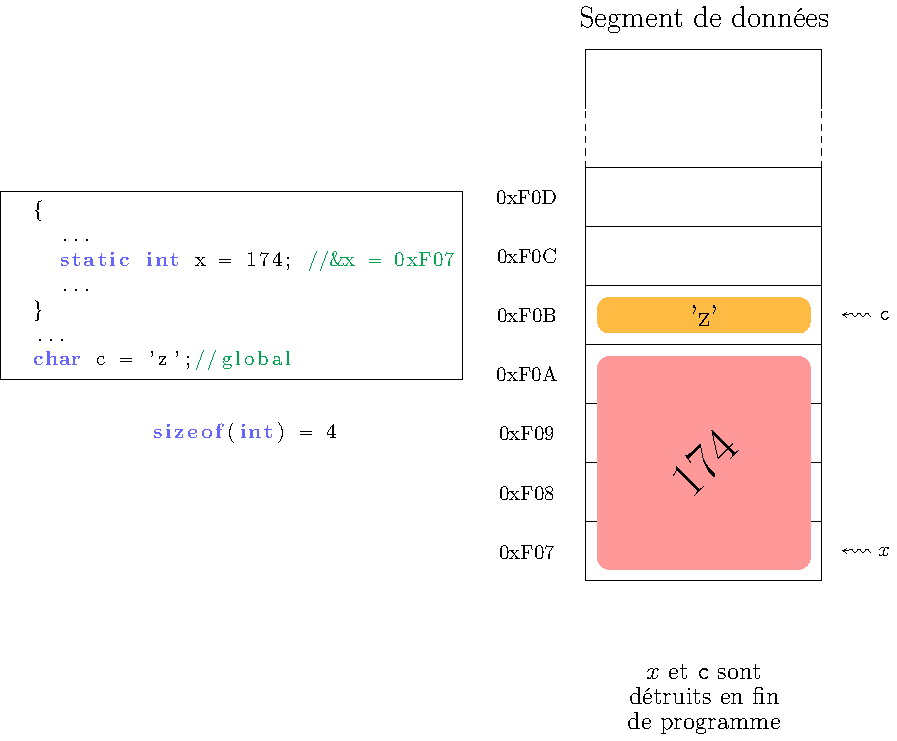
\includegraphics[height=7cm]{pics/static.pdf}
\end{center}
\end{frame}

\begin{frame}
\frametitle{Métaphore}
\begin{itemize}[<+->]
\item Enregistrer des données dans le segment de données est comme mettre des marchandises dans un gros sac sous vide
	\begin{itemize}
	\item La taille du sac est exactement celle des marchandises stockées
		\begin{itemize}
		\item Taille du segment = somme des tailles des données
		\end{itemize}
	\item Les marchandises sont les unes à côté des autres, il n'y a pas d'espace libre
		\begin{itemize}
		\item Données contiguës en mémoire
		\end{itemize}
	\end{itemize}
\end{itemize}
\begin{alertblock}<+->{Attention}
	\begin{itemize}[<+->]
	\item \lstinline|static| en \java\ a donc une signification très différente en \texttt{C} / \cpp.
	\item Les « constantes » globales déclarées avec \lstinline|\#define| \emph{ne} sont \emph{pas} allouées
	\end{itemize}
\end{alertblock}
\end{frame}

\begin{frame}[containsverbatim]
\frametitle{Exemple 1}
\begin{itemize}
\item Fichier \texttt{static.cpp}
\end{itemize}
\begin{lstlisting}
const double PI = 3.14;

double circle_area(double r)
{
	return PI * r * r;
}

int main()
{
	cout << circle_area(2) << endl;
}
\end{lstlisting}
\end{frame}

\begin{frame}[containsverbatim]
\frametitle{Exemple 2}
\begin{itemize}
\item Fichier \texttt{static.cpp}
\end{itemize}
\begin{lstlisting}
int countDown()
{
	static int i = 6;	
	i--;
	return i;
}

void boom()
{
	bool stop = false;
	while(! stop)
	{
		int j = countDown();
		if(j >= 0)
			cout << j << endl;
		else
			stop = true;
	}
	cout << "BOOM" << endl;		
}

int main()
{
	boom();
}
\end{lstlisting}
\end{frame}

\begin{frame}
\frametitle{Avantages et inconvénients}
\begin{block}<+->{Avantages}
	\begin{itemize}[<+->]
	\item Allocation très rapide
	\item Portée illimitée
	\item Durée de vie illimitée
	\end{itemize}
\end{block}
\begin{alertblock}<+->{Inconvénients}
	\begin{itemize}[<+->]
	\item Portée (semi) globale
		\begin{itemize}
		\item Organisation de code
		\end{itemize}
	\item Durée de vie illimitée
	\end{itemize}
\end{alertblock}
\end{frame}

\begin{frame}
\frametitle{Remarques à propos du segment de données}
\begin{itemize}[<+->]
\item La mémoire est allouée tant qu'il reste de la place dans le segment de données
	\begin{itemize}
	\item La taille maximale du segment de donnée est déterminée par le système (\texttt{ulimit -d})
	\item S'il n'y a plus de place, l'allocation est rejetée	
	\end{itemize}
\item Le segment de donnée n'est pas « protégé » par la portée
	\begin{itemize}
	\item Le programmeur est responsable de son utilisation
	\end{itemize}
\end{itemize}
\begin{block}<+->{Hygiène de programmation}
	\begin{itemize}
	\item Éviter en \cpp
	\end{itemize}
\end{block}
\end{frame}

\begin{frame}[containsverbatim]
\frametitle{Exemple de bonne utilisation}
\begin{itemize}
\item Fichier \texttt{good-static.c}
\end{itemize}
\begin{lstlisting}
const char * policy = "azertyuiopqsdfghjklmwxcvbn0123456789!?.";
//unsigned l = strlen(policy); //can't do

unsigned policy_length()
{
    static unsigned length = 0;
    static bool computed = false; //did I already compute length ?
    
    if(! computed)
    {
        length = strlen(policy);
        computed = true;
    }
    
    return length;
}
\end{lstlisting}
\begin{itemize}
\item Les variables \texttt{length} et \texttt{computed} sont instanciées et initialisées une unique fois
\item Ils sont réutilisés à chaque appel de \texttt{policy\_length}
\end{itemize}
\end{frame}

\section{Allocation automatique}

\begin{frame}
\frametitle{Classe d'allocation automatique}
\begin{itemize}[<+->]
\item Variables non globales allouées sans mot-clé ou locales avec \lstinline|auto|, à la déclaration
\item Portée toujours locale
\item Durée de vie
	\begin{itemize}
	\item Mémoire allouée à la déclaration
	\item Mémoire désallouée automatiquement en fin de bloc
	\end{itemize}
\item Valeurs par défaut
	\begin{itemize}
	\item Aucune (valeur indéterminée)
	\end{itemize}
\item Habituellement, les données sont stockées sur la pile
	\begin{itemize}
	\item Stockées au sommet de la pile 
		\begin{itemize}
		\item Registre \texttt{rsp}, adresses décroissantes
		\end{itemize}
%	\item La taille maximale de la pile a une valeur déterminée à la compilation // wtf ?!
	\item Le plus grand espace allouable est déterminé par le système
	\item Haute performance : on sait \emph{à la compilation} où stocker
		\begin{itemize}
		\item Pas de calcul ou d'appel système nécessaire à l'exécution
		\end{itemize}
	\item L'affectation des données est au pire réalisée à l'exécution
	\end{itemize}
\end{itemize}
\end{frame}

\begin{frame}
\frametitle{Illustration}
\begin{center}
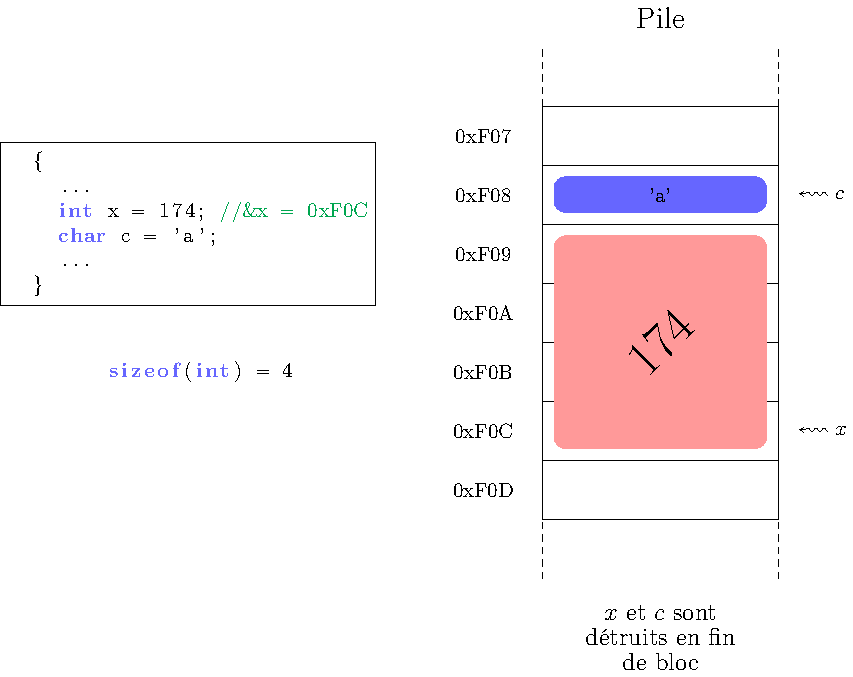
\includegraphics[height=7cm]{pics/automatic.pdf}
\end{center}
\end{frame}

\begin{frame}
\frametitle{Métaphore}
\begin{itemize}[<+->]
\item Enregistrer des données sur la pile est comme stocker des caisses au fond d'un puits
	\begin{itemize}
	\item Pour stocker, on lâche la caisse qui tombe au fond du puits
		\begin{itemize}
		\item Données enregistrées au sommet de la pile
		\end{itemize}
	\item On sait \emph{a priori} où va la caisse
		\begin{itemize}
		\item À la compilation, on sait où la donnée est enregistrée
		\item Au sommet de la pile, relativement à \texttt{rsp}
		\end{itemize}
	\item Très rapide de stocker : on lâche la caisse
		\begin{itemize}
		\item Aucun calcul n'est effectué à l'exécution
		\end{itemize}
	\end{itemize}
\item En \java, seuls les primitifs et les adresses d'objets sont alloués sur la pile
\end{itemize}
\end{frame}

\begin{frame}[containsverbatim]
\frametitle{Exemple}
\begin{itemize}
\item Fichier \texttt{automatic.cpp}
\end{itemize}
\begin{lstlisting}
int main()
{
	int i = 5; //most likely on stack
	while(i >= 0)
	{
		int j = i + 2; //most likely on stack
		
		cout << i << " " << j << endl;

		i--;
	}//j is destroyed
	cout << i << endl;
	//cout << j << endl;//j is out of the scope
}//i is destroyed
\end{lstlisting}
\end{frame}

\begin{frame}[containsverbatim]
\frametitle{Exemple 2}
\begin{itemize}
\item Fichier \texttt{automatic2.cpp}
\end{itemize}
\begin{lstlisting}
int explodeStack(int i)
{	
	int j = i * 2; //creates j most likely on the stack

	if(i != 1)
		explodeStack(j); //backup registers on stack and call (infinite recursion)
}

int main()
{
	explodeStack(10);
}
\end{lstlisting}
\end{frame}

\begin{frame}
\frametitle{Avantages et inconvénients}
\begin{block}<+->{Avantages}
	\begin{itemize}[<+->]
	\item Allocation rapide
	\item Portée limitée
	\item Durée de vie limitée
	\item Allocation et désallocation implicite
	\end{itemize}
\end{block}
\begin{alertblock}<+->{Inconvénients}
	\begin{itemize}[<+->]
	\item Portée limitée		
	\item Durée de vie limitée	
	\end{itemize}
\end{alertblock}
\end{frame}

\begin{frame}
\frametitle{Remarques à propos de la pile}
\begin{itemize}[<+->]
\item La mémoire est allouée tant qu'il reste de la place dans la pile
	\begin{itemize}
	\item La taille maximale de la pile est déterminée par le système (\texttt{ulimit -s})
	\item S'il n'y a plus de place, l'allocation est rejetée	
	\end{itemize}
\item La pile n'est pas protégée en écriture (pour un même programme)
	\begin{itemize}
	\item Le programmeur est responsable de son utilisation
	\item Une sortie de tableau peut corrompre son état
		\begin{itemize}
		\item Variables corrompues
		\item Pile d'exécution corrompue
		\end{itemize}
	\end{itemize}
\end{itemize}
\begin{block}<+->{Hygiène de programmation}
	\begin{itemize}
	\item Utiliser au maximum en \cpp
	\end{itemize}
\end{block}
\end{frame}

\section{Allocation dynamique}

\begin{frame}
\frametitle{Classe d'allocation dynamique (1/2)}
\begin{itemize}[<+->]
\item Allocation avec \lstinline|new| / \texttt{malloc} et destruction avec \lstinline|delete| / \texttt{free}
	\begin{itemize}
	\item Allouent un espace mémoire et retournent l'adresse vers l'espace alloué
	\item L'adresse des données est en classe automatique
	\item Les données sont en classe dynamique
	\end{itemize}
\item Portée
	\begin{itemize}
	\item l'adresse allouée de la donnée est locale au bloc
	\item les données sont accessibles globalement via leur adresse
	\end{itemize}
\item Les données sont habituellement stockées dans le tas
	\begin{itemize}
	\item Ces données ne sont pas contiguës en mémoire
	\item L'endroit où sont stockées les données est déterminé à l'exécution
	\item Le stockage des données est réalisé à l'exécution
	\item Performance plus faible : appel système est effectué (à l'exécution) pour déterminer où stocker les données
	\end{itemize}
\end{itemize}
\end{frame}

\begin{frame}
\frametitle{Classe d'allocation dynamique (2/2)}
\begin{itemize}[<+->]
\item Durée de vie
	\begin{itemize}
	\item Mémoire allouée à l'instanciation par \lstinline|new| / \texttt{malloc}
		\begin{itemize}
		\item À la compilation, on sait où va l'adresse des données allouées
		\item ... mais pas les données allouées
		\end{itemize}
	\item L'adresse des données est désallouée en sortie de bloc
		\begin{itemize}
		\item Car elle est de classe automatique
		\end{itemize}
	\item Mémoire désallouée explicitement par \lstinline|delete| / \texttt{free}
		\begin{itemize}
		\item Si on ne le fait pas : fuite mémoire
		\item Les ressources sont \emph{perdues}
		\item Le système d'exploitation \emph{devrait} désallouer en fin de programme
		\end{itemize}
	\end{itemize}
\item Valeurs par défaut
	\begin{itemize}
	\item Aucune : instanciation explicite nécessaire
	\end{itemize}
\end{itemize}
\end{frame}

\begin{frame}
\frametitle{Illustration}
\begin{center}
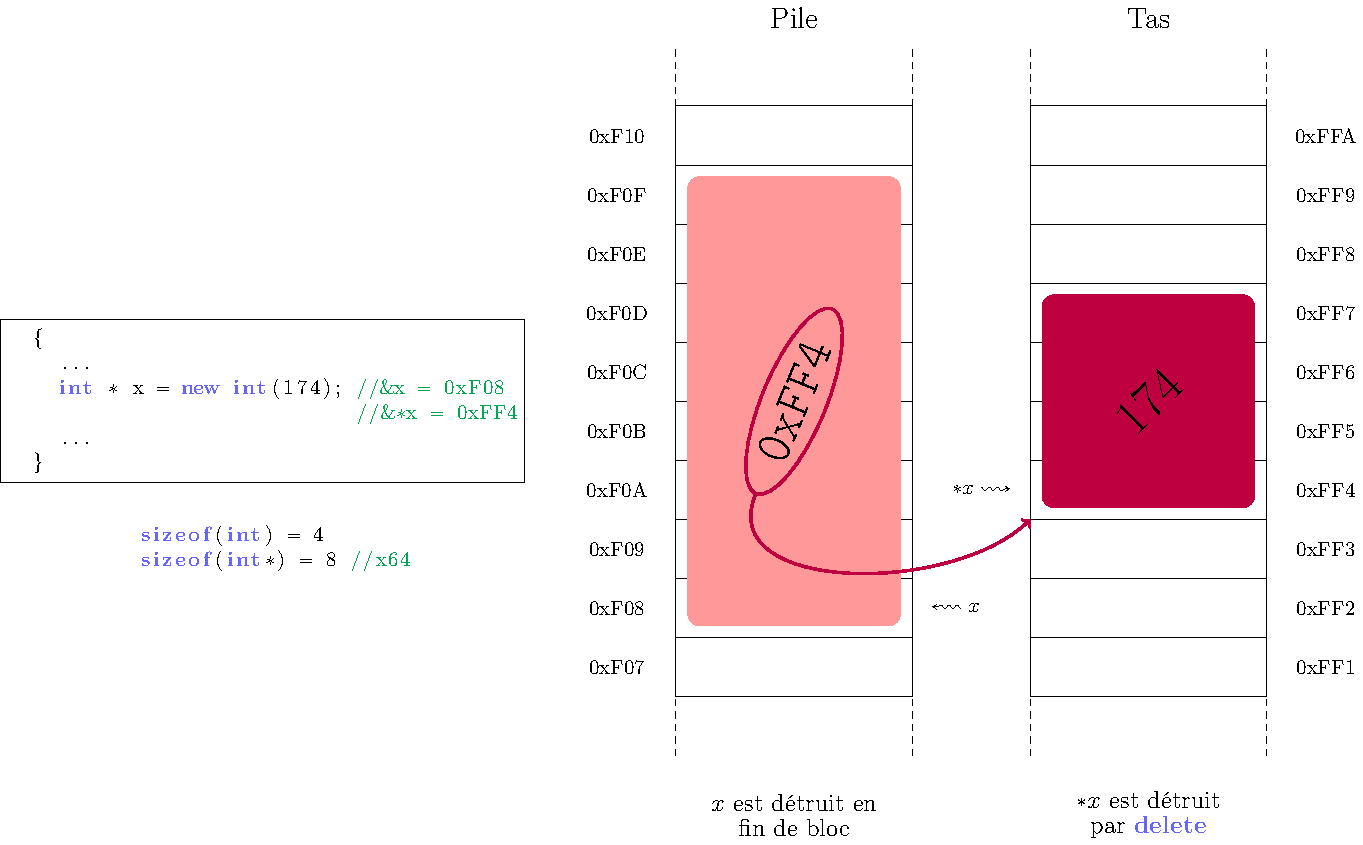
\includegraphics[height=7cm]{pics/dynamic.pdf}
\end{center}
\end{frame}

\begin{frame}
\frametitle{Métaphore}
\begin{itemize}[<+->]
\item Enregistrer des données dans le tas est comme stocker des marchandises dans un entrepôt
	\begin{enumerate}
	\item Quand on veut stocker des marchandises, on demande au concierge si c'est possible
		\begin{itemize}
		\item Appel système effectué pour l'allocation
		\end{itemize}
	\item Le concierge cherche un endroit dans l'entrepôt où stocker
		\begin{itemize}
		\item Le système d'exploitation cherche un espace mémoire libre
		\end{itemize}
	\item S'il y a de la place, le concierge stocke la caisse et donne un ticket décrivant où elle est stockée
		\begin{itemize}
		\item Le système d'exploitation alloue un espace mémoire et retourne l'adresse de cet espace
		\end{itemize}
	\item S'il n'y a pas de place : ko
		\begin{itemize}
		\item Cela ne veut pas dire que la mémoire est saturée
		\item Elle est peut-être simplement fragmentée
		\end{itemize}
	\end{enumerate}
\end{itemize}
\end{frame}

\begin{frame}
\frametitle{Fonction d'allocation dynamique en \texttt{C}}
\begin{enumerate}[<+->]
\item \texttt{malloc(size\_t)} : alloue la mémoire sur le tas
	\begin{itemize}
	\item Retourne l'adresse vers l'espace alloué
	\item La mémoire a une valeur indéterminée
	\end{itemize}
\item \texttt{calloc(size\_t n, size\_t m)} : alloue des « tableaux »
	\begin{itemize}
	\item Mets la mémoire à zéro
	\item À cause de l'alignement, la taille allouée n'est pas toujours $nm$
	\end{itemize}	
\item \texttt{realloc(void*, size\_t)} : réalloue de la mémoire préalablement allouée par \texttt{malloc}, \texttt{calloc} ou \texttt{realloc}
	\begin{itemize}
	\item Contracte ou étend un emplacement
	\item Déplacement / copie possible
	\end{itemize}
\end{enumerate}
\begin{alertblock}<+->{Remarque importante}
	\begin{itemize}[<+->]
	\item Avec \texttt{realloc}, si l'allocation échoue, l'ancien emplacement \emph{n'est pas libéré}
	\end{itemize}
\end{alertblock}
\begin{itemize}[<+->]
\item Nécessaire d'inclure \texttt{stdlib.h}
\end{itemize}
\end{frame}

\begin{frame}[containsverbatim]
\frametitle{Exemple \cpp}
\begin{itemize}
\item Fichier \texttt{dynamic-cpp.cpp}
\end{itemize}
\begin{lstlisting}
int main()
{
	Point * p = new Point(2,3);
	cout << p->getX() << " " << p->getY() << endl;
	delete p;
	cout << p->getX() << " " << p->getY() << endl;//unpredictable is p is deleted
	
	Point * p2 = nullptr;
	Point * pp2 = nullptr;
	Point p3;//(0,0)

	{
		p2 = new Point(3,4);
		cout << p2->getX() << " " << p2->getY() << endl;
		pp2 = p2;
		p3 = *p2;		
		//delete p2;//uncomment
	}

	cout << p2->getX() << " " << p2->getY() << endl;
	cout << pp2->getX() << " " << pp2->getY() << endl;		
	cout << p3.getX() << " " << p3.getY() << endl;		
} 	//Q : does it leak ?
\end{lstlisting}
\end{frame}

\begin{frame}[containsverbatim]
\frametitle{Exemple \texttt{C}}
\begin{itemize}
\item Fichier \texttt{dynamic-c.cpp}
\end{itemize}
\begin{lstlisting}
int main()
{
    Point * p = (Point*) malloc(sizeof(Point));
    p->x = 1; p->y = 2;   
    print_point(*p);
    
    free(p);
    print_point(*p);
    
    Point * p2 = NULL; Point * pp2 = NULL;    
    Point p3;

    {
        p2 = (Point*) malloc(sizeof(Point)); 
        p2->x = 3; p2->y = 4;
        print_point(*p2);
        pp2 = p2;

        p3 = *p2;		
        //free(p2); //uncomment
    }

    print_point(*p2);
    print_point(*pp2);
    print_point(p3);	
}
\end{lstlisting}
\end{frame}

\begin{frame}[containsverbatim]
\frametitle{Illustration des fonctions d'allocation en \texttt{C} (1/2)}
\begin{itemize}
\item Fichier \texttt{fct-alloc-c.c}
\end{itemize}
\begin{lstlisting}
int main()
{
    int * p = (int*) malloc(4 * sizeof(int));
    print_int_array(p, 4); //undeterminate values
    
    free(p);
    print_int_array(p, 4); //undefined behaviour
    
    p = (int*) calloc(4, sizeof(int));
    print_int_array(p, 4); //0 0 0 0
    
    for(int i = 0; i < 4; i++)
        p[i] = i;
    print_int_array(p, 4); //0 1 2 3
}
\end{lstlisting}
\end{frame}

\begin{frame}[containsverbatim]
\frametitle{Illustration des fonctions d'allocation en \texttt{C} (2/2)}
\begin{itemize}
\item Fichier \texttt{fct-alloc-c.c}
\end{itemize}
\begin{lstlisting}
int main()
{
    int * p = (int*) malloc(4 * sizeof(int));

    p = (int*) realloc(p, 2 * sizeof(int));
    if(p) //check wether allocation suceeded
    {
        print_int_array(p, 2); //0 1
        print_int_array(p, 4); //0 1 2 3 : not undeterminate
    }
    else
        free(p);
    
    p = (int*) realloc(p, 4 * sizeof(int));
    if(p)
    {
        print_int_array(p, 2); //0 1
        print_int_array(p, 4); //0 1 ? ?
    }
    else
        free(p);
}
\end{lstlisting}
\end{frame}

\begin{frame}[containsverbatim]
\frametitle{Exemple}
\begin{itemize}
\item Fichier \texttt{paginate.cpp}
\end{itemize}
\begin{lstlisting}
int main()
{		
	long long unsigned int j = 0;
	while(true)//this is going to hurt
	{
		new int[250];//should weight 1kb
		j++;
		if(j % 100 == 0)
			cout << j << "kb allocated" << endl;		
	}
}	
\end{lstlisting}
\end{frame}

\begin{frame}
\frametitle{Rappel sur les pointeurs}
\begin{itemize}[<+->]
\item Les pointeurs \emph{sont} des adresses
\item Ces adresses peuvent correspondre à un espace alloué, ou non
\item Accéder à un espace qui n'a pas été alloué amène à un comportement indéterminé
	\begin{itemize}
	\item Zéro
	\item Ancienne valeur
	\item Erreur de segmentation
	\end{itemize}
\item Affecter une valeur à un pointeur change la valeur de l'adresse
	\begin{itemize}
	\item Pas ce que pointe l'adresse
	\end{itemize}
\item Pour changer ce qui est pointé, il faut déférencer 
	\begin{itemize}
	\item \texttt{*pt = 42;}
	\end{itemize}
\end{itemize}
\end{frame}

\begin{frame}
\frametitle{Exemple}
\begin{itemize}[<+->]
\item \lstinline|int * pt = 3;|
	\begin{enumerate}
	\item Alloue un espace de 8 bytes (x64) sur la pile
	\item Donne à cet espace la valeur \texttt{0x00\_00\_00\_00\_00\_00\_00\_03}
	\item L'instruction \lstinline|int i = *pt;| provoque probablement une erreur de segmentation
	\end{enumerate}
\item \lstinline|int * pt = NULL;| et \lstinline|int * pt = nullptr| se comportent de la même manière
	\begin{itemize}
	\item Erreurs de segmentation au déférencement
	\end{itemize}
\item \lstinline|int * pt = (int*)malloc(sizeof(int)); *pt = 3;|
	\begin{enumerate}
	\item Alloue un espace \texttt{pt} de 8 bytes (x64) sur la pile
	\item Alloue un espace $s$ de \lstinline|sizeof(int)| sur le tas
	\item Affecte à \texttt{pt} l'adresse de $s$
	\item Affecte à l'adresse pointée par \texttt{pt} (dans $s$) la valeur $3$
	\end{enumerate}
\item \lstinline|int * pt = new int(3);| est l'équivalent en \cpp
\end{itemize}
\end{frame}

\begin{frame}
\frametitle{Avantages et inconvénients}
\begin{block}<+->{Avantages}
	\begin{itemize}[<+->]
	\item Portée relativement illimitée
	\item Durée de vie illimitée
	\item Émulation de passage par référence
	\item Possibilité d'allouer de larges quantité de mémoire
	\end{itemize}
\end{block}
\begin{alertblock}<+->{Inconvénients}
	\begin{itemize}[<+->]
	\item Allocation plus lente
	\item Destruction manuelle nécessaire
		\begin{itemize}
		\item Attention aux fuites mémoires et double free
		\end{itemize}
	\item Autres contraintes (copie, affectation)
	\end{itemize}
\end{alertblock}
\end{frame}

\begin{frame}
\frametitle{Remarques}
\begin{itemize}[<+->]
\item La mémoire est allouée tant qu'il reste de la place en mémoire
	\begin{itemize}
	\item La taille maximale du tas est déterminée par le système
		\begin{itemize}
		\item S'il n'y a plus de place (\texttt{ulimit -m}), l'allocation est rejetée	
		\item S'il n'y a plus de place en mémoire, les mécanismes de \texttt{swap} et de pagination du système \emph{devraient} prendre le relais 
		\end{itemize}
	\end{itemize}
\item La mémoire n'est pas protégée en écriture (pour un même programme)
	\begin{itemize}
	\item Le programmeur est responsable de son utilisation
	\item Une sortie de tableau peut corrompre son état
		\begin{itemize}
		\item Variables corrompues
		\end{itemize}
	\end{itemize}
\end{itemize}
\begin{block}<+->{Hygiène de programmation}
	\begin{itemize}
	\item Limiter son utilisation \cpp
	\end{itemize}
\end{block}
\end{frame}

\begin{frame}
\frametitle{Risques liés à \texttt{new} / \texttt{malloc}}
\begin{enumerate}[<+->]
\item Il faut libérer manuellement toute mémoire allouée
	\begin{itemize}
	\item Sinon, il y a une fuite mémoire
	\item La mémoire n'est pas toujours libérée dans le scope ou la classe où elle est allouée
	\item Risque de double \lstinline|delete| / \texttt{free}: erreur de segmentation
	\end{itemize}
\item Un pointeur (en particulier ceux issus de \lstinline|new| / \texttt{malloc}) peut être \lstinline|NULL| ou \lstinline|nullptr|
	\begin{itemize}
	\item Pas une référence
	\end{itemize}
\item En cas d'allocation dynamique pour un attribut de classe, il faut prendre des précautions particulières
	\begin{enumerate}
	\item Destructeur
	\item Constructeur de recopie (cf. Chapitre 8)
	\item Opérateur d'affectation (cf. Chapitre 8)
	\end{enumerate}
\end{enumerate}
\end{frame}

\begin{frame}
\frametitle{Utilisation de \texttt{new} / \texttt{malloc}}
\begin{itemize}[<+->]
\item En \texttt{C}, utiliser l'allocation dynamique est parfois indispensable
	\begin{itemize}
	\item Cf. section suivante
	\end{itemize}
\end{itemize}
\begin{alertblock}<+->{Je veux faire un \texttt{new} en \cpp}
	\begin{itemize}[<+->]
	\item \textcolor{esi-red}{\Huge{\textsc{Non !}}}
	\end{itemize}
\end{alertblock}
\end{frame}

\begin{frame}
\frametitle{Utilisation de \texttt{new} en \cpp}
\begin{exampleblock}<+->{Je veux quand même faire un \texttt{new}}
	\begin{enumerate}[<+->]
	\item J'ai l'habitude en \java
%		\begin{itemize}
%		\item On n'est pas en \java. 
			\begin{itemize}
			\item En \java, on ne peut pas écrire sur la pile
			\item En \java, il y a un garbage collector (compromis efficacité / sûreté)
			\end{itemize}
%		\end{itemize}
	\item Je veux éviter une copie de paramètre de fonction
		\begin{itemize}
		\item Utilise le passage par référence
		\end{itemize}
	\item Je veux qu'une fonction modifie ses paramètres (effet de bord)
		\begin{itemize}
		\item Utilise le passage par référence
		\end{itemize}
	\item Je veux avoir un attribut sans avoir à le recopier par le constructeur
		\begin{itemize}
		\item Utilise une référence
		\end{itemize}
	\item Je veux activer le polymorphisme
		\begin{itemize}
		\item Utilise une référence
		\end{itemize}
	\end{enumerate}
\end{exampleblock}
\end{frame}

\begin{frame}
\frametitle{Moralité}
\begin{block}<+->{Hygiène de programmation en \cpp}
	\begin{itemize}[<+->]
	\item Utilisez des références quand vous pouvez
	\item Utilisez des pointeurs quand vous devez
	\end{itemize}
\end{block}
\begin{itemize}[<+->]
\item Exemple d'obligation : résoudre une dépendance cyclique
\end{itemize}
\begin{exampleblock}<+->{Si on veut \emph{vraiment} utiliser \texttt{new}}
	\begin{itemize}[<+->]
	\item Encapsulation dans des \emph{pointeurs intelligents}
	\end{itemize}
\end{exampleblock}
\begin{itemize}[<+->]
\item Cf. fin de chapitre
\end{itemize}
\end{frame}

\section{Portée et durée de vie}

\begin{frame}
\frametitle{Récapitulatifs}
\begin{itemize}[<+->]
\item En \texttt{C} / \cpp, pas de notion de segment de données, pile ou tas
\item Les classes d'allocation ne définissent que la durée de vie
\item Allocation statique
	\begin{itemize}[<+->]
	\item Portée locale ou globale
	\item Alloué en début de programme, détruit à la fin
	\end{itemize}
\item Allocation automatique
	\begin{itemize}
	\item Portée locale
	\item Alloué à la déclaration, désalloué en sortie de bloc
	\end{itemize}
\item Allocation dynamique
	\begin{itemize}
	\item Portée « locale / globale »
	\item Alloué et désalloué explicitement
	\end{itemize}
\end{itemize}
\end{frame}

\begin{frame}[containsverbatim]
\frametitle{Illustration en \texttt{C}}
\begin{itemize}
\item Fichier \texttt{life.c}
\end{itemize}
\begin{lstlisting}
int * addr_auto, * addr_dyn, * addr_stat = NULL; //statiques, globales
int global = 2; //statique, globale

int f() {
	int j = 42; //automatique, locale à f
	addr_auto = &j; //ok
	int * pt = (int*)malloc(sizeof(int)); //dynamique, locale
    *pt = 23; //ok : espace alloué
	addr_dyn = pt; //ok
    static int l = 17; //statique, locale
    addr_stat = &l;
	global = 3;
} //j et pt sont désalloués (mais pas *pt, ni l)

int main() {
	f();
    printf("%p:", addr_auto); //ok (dangling)
    printf("%d\n", *addr_auto); //KO : j est désaloué	
    printf("%p:", addr_dyn); //ok
    printf("%d\n", *addr_dyn); //ok : *addr_dyn n'a pas été désalloué	
    printf("%p:", addr_stat); //ok
    printf("%d\n", *addr_stat); //ok : l n'a pas été désalloué
    printf("%d\n", global); //ok    
    
    free(addr_dyn);
    printf("%p:", addr_dyn); //ok (dangling)
    printf("%d\n", *addr_dyn); //KO : *addr_dyn est désalloué	    
}
\end{lstlisting}
\end{frame}

\begin{frame}[containsverbatim]
\frametitle{Illustration en \cpp}
\begin{itemize}
\item Fichier \texttt{life.cpp}
\end{itemize}
\begin{lstlisting}
int *pt1, *pt2, *pt3 = nullptr; //statiques, globales
int global = 2; //statique, globale

int f()
{
	int j = 42; //automatique, locale à f
	pt1 = &j; //ok
	int * k = new int(23); //dynamique, locale
	pt2 = k; //ok
	static int l = 17; //statique, locale
	pt3 = &l;
	global = 3;
} //j et k sont désalloués (mais pas *k, ni l)

int main()
{
	f();
	cout << pt1 << ":"; //ok
	cout << *pt1 << endl; //ko : j est désaloué
	cout << pt2 << ":"; //ok
	cout << *pt2 << endl; //ok : *k n'a pas été désalloué
	cout << pt3 << ":"; //ok
	cout << *pt3 << endl; //ok : l n'a pas été désalloué
	cout << global << endl; //ok
}
\end{lstlisting}
\end{frame}

\begin{frame}
\frametitle{Le cas des classes}
\begin{itemize}[<+->]
\item Souvent, l'adresse d'un objet est l'adresse du premier attribut
\item Les attributs non dynamiques et non statiques ont la même classe d'allocation que l'objet
\item Les attributs \lstinline|static| sont statiques
\item Attributs dynamiques
	\begin{itemize}
	\item Données en classe d'allocation dynamique
	\item Adresses de même classe d'allocation que l'objet
	\end{itemize}
\item Les fonctions membres sont généralement allouées dans le segment de code
	\begin{itemize}
	\item Pas les fonctions \lstinline|inline|
	\end{itemize}
\item Les remarques en terme de portée et de durée de vie sont valides sous ces conditions
\end{itemize}
\end{frame}

\begin{frame}[containsverbatim]
\frametitle{Illustration}
\begin{itemize}
\item Fichier \texttt{class-alloc.cpp}
\end{itemize}
\begin{lstlisting}
struct Array {
    int i;
    int * arr;
    
    Array(int i) : i(i) {
        arr = new int[i];
    }    
}; //missing destructor... and other things

int main() {
    Array a(2); //a automatic
                //i automatic
                //tab automatic
                //*tab dynamic    
    
    static Array b(2); //b static
                       //i static
                       //tab static
                       //*tab dynamic

    Array * c = new Array(2); //c dynamic
                              //i dynamic
                              //tab dynamic
                              //*tab dynamic
}
\end{lstlisting}
\end{frame}

\begin{frame}
\frametitle{Les doubles pointeurs en \texttt{C}}
\begin{itemize}[<+->]
\item En \texttt{C}, on a parfois besoin d'utiliser des doubles pointeurs
	\begin{itemize}
	\item Classiquement, lorsque l'on dissocier des allocations
	\end{itemize}
\end{itemize}
\begin{exampleblock}<+->{Exemple}
	\begin{itemize}[<+->]
	\item On veut créer une fonction qui alloue un tableau d'entiers
	\item On peut soit
		\begin{itemize}
		\item laisser le compilateur créer le pointeur qui contiendra l'adresse de l'espace alloué
		\item fournir le pointeur qui contiendra l'adresse de l'espace alloué		
		\end{itemize}
	\end{itemize}
\end{exampleblock}
\begin{itemize}[<+->]
\item Parfois, l'application que l'on fait des pointeurs «~force~» le programmeur à le fournir
\end{itemize}
\end{frame}

\begin{frame}[containsverbatim]
\frametitle{Idée stupide}
\begin{itemize}
\item On retourne l'adresse d'une variable locale
\end{itemize}
\begin{lstlisting}
int* allocate_auto(int size)
{
    int tab[size];
    for(int i = 0; i < size; i++)
		tab[i] = i;
    return tab;
}
\end{lstlisting}
\begin{itemize}
\item Erreur de segmentation !
\item Fichier \texttt{doubleptr.c}
\end{itemize}
\end{frame}


\begin{frame}[containsverbatim]
\frametitle{Premier cas : on laisse le compilateur faire}
\begin{enumerate}
\item On déclare le pointeur, on alloue et on affecte le pointeur avec \texttt{malloc}
\item On affecte l'espace alloué avec l'opérateur \texttt{[]}
\item On retourne le pointeur
\end{enumerate}
\begin{lstlisting}
int* allocate(int size)
{
	int* pt = (int*)malloc(size * sizeof(int));
	for(int i = 0; i < size; i++)
		pt[i] = i; //*(pt + i * sizeof(int)) si pt est void*

	return pt;
}

int main()
{
	int * pt = allocate(5); //crée un pointeur pour stocker 5 entiers
	for(int i = 0; i < 5; i++)
		printf("%d ", pt[i]);
	printf("\n");

	free(pt);
}
\end{lstlisting}
\end{frame}

\begin{frame}[containsverbatim]
\frametitle{Deuxième cas : on fournit le pointeur}
\begin{enumerate}
\item On déclare le pointeur dans \texttt{main}, on alloue et on affecte le pointeur avec \texttt{malloc} dans une fonction
\item On affecte l'espace alloué en déférençant le pointeur
\item On retourne le pointeur
\end{enumerate}
\begin{lstlisting}
void allocate(int* pt, int size)
{
	pt = (int*)malloc(size * sizeof(int));
	for(int i = 0; i < size; i++)
		pt[i] = i;
}

int main()
{
	int * pt = NULL;
	allocate(pt, 5);
	for(int i = 0; i < 5; i++)
		printf("%d ", pt[i]);
	printf("\n");

	free(pt);
}
\end{lstlisting}
\begin{itemize}
\item Erreur de segmentation !
\end{itemize}
\end{frame}

\begin{frame}[<+->]
\frametitle{Le nœud du problème}
\begin{enumerate}[<+->]
\item On crée \texttt{pt} dans \texttt{main}
\item On lui affecte la valeur \texttt{NULL}
	\begin{itemize}
	\item Macro, valeur zéro
	\end{itemize}
\item On appelle \texttt{allocate} en passant \texttt{pt} en paramètre
\item \texttt{pt} est passé par \emph{valeur}
	\begin{itemize}
	\item On passe une copie \texttt{pt'} de \texttt{pt} à \texttt{allocate}
	\end{itemize}
\item On alloue un espace dans \texttt{allocate}, et on affecte \texttt{pt'} à l'adresse de cet espace
\item On affecte des valeurs dans l'espace alloué
\item On retourne dans \texttt{main}
	\begin{itemize}
	\item \texttt{pt} est toujours à \texttt{NULL}
	\end{itemize}
\item On déférence \texttt{pt}
\item Erreur de segmentation
\end{enumerate}
\end{frame}

\begin{frame}
\frametitle{Solution}
\begin{exampleblock}<+->{Idée}
	\begin{itemize}[<+->]
	\item Il faudrait passer \texttt{pt} par adresse
	\end{itemize}
\end{exampleblock}
\begin{itemize}[<+->]
\item Il faut donc prendre l'adresse d'un pointeur
	\begin{itemize}
	\item L'adresse d'un type \texttt{T} est de type \texttt{T*}
	\item L'adresse d'un type \texttt{T*} est de type \texttt{T**}
	\end{itemize}
\item Double pointeur
\item En \cpp, les doubles pointeurs sont très souvent inutiles car on possède les références
	\begin{itemize}
	\item On évite d'utiliser une grande quantité de pointeurs grâce à ce concept
	\end{itemize}
\end{itemize}
\end{frame}

\begin{frame}[containsverbatim]
\frametitle{Deuxième cas bis : on utilise un double pointeur}
\begin{enumerate}
\item On déclare le pointeur dans \texttt{main}, on le passe par adresse à \texttt{allocate}
\item On affecte l'espace alloué en déférençant l'adresse du pointeur
	\begin{itemize}
	\item Ainsi, on a un effet de bord dans \texttt{main}
	\end{itemize}
\end{enumerate}
\begin{lstlisting}
void allocate(int** pt, int size)
{
	*pt = (int*)malloc(size * sizeof(int));
	for(int i = 0; i < size; i++)
		(*pt)[i] = i;
}

int main()
{
	int * pt = NULL;
	allocate(&pt, 5);
	for(int i = 0; i < 5; i++)
		printf("%d ", pt[i]);
	printf("\n");

	free(pt);
}
\end{lstlisting}
\begin{itemize}
\item Fichier \texttt{double-ptr.c}
\end{itemize}
\end{frame}

\section{Pointeurs intelligents}

\begin{frame}
\frametitle{Nécessité en allocation dynamique}
\begin{itemize}[<+->]
\item Quand on sort d'un scope, il faut décider quoi faire de la mémoire allouée
\item Utilisation du patron de classe, \texttt{unique\_ptr}, \texttt{shared\_ptr} et \texttt{weak\_ptr}.
\item Paramétré par le type de la variable dynamique à encapsuler
\item Comportements « similaires » aux pointeurs / références, en classe automatique, implémenté via un patron de classe et la surcharge d'opérateurs (cf. Ch. 7).
\item Chaque patron définit comment la mémoire doit être gérée à la destruction (automatique) du pointeur intelligent.
	\begin{itemize}
	\item On détruit les données ?
	\item On détruit les données si plus rien ne pointe dessus ?
	\item On ne détruit rien ?
	\end{itemize}
\item Implémenté en comptant le nombre de références dans le constructeur à l'aide d'une variable statique.
\item Inclure \texttt{memory.h} (\cpp uniquement)
\end{itemize}
\end{frame}

\begin{frame}
\frametitle{Pointeurs intelligents}
\begin{itemize}[<+->]
\item Quand un pointeur possédant un objet est détruit, il faut définir comment libérer la mémoire
%\item En particulier, on veut
%	\begin{enumerate}
%	\item Éviter les fuites mémoires
%	\item Éviter les double \texttt{delete}
%	\end{enumerate}
\item Trois types de pointeurs intelligents « principaux »
	\begin{enumerate}
	\item \texttt{unique\_ptr} : pointeur intelligent qui n'autorise qu'une possession unique de l'objet. 
		\begin{itemize}
		\item Copier et affecter le pointeur provoque une erreur de compilation.
		\item Quand le pointeur est détruit, la donnée est détruite.
		\end{itemize}
	\item \texttt{shared\_ptr} : pointeur intelligent qui autorise des possessions multiples d'un même objet.
		\begin{itemize}
		\item Les données pointées sont détruites si plus rien ne pointe dessus.
		\item Le dernier pointeur possédant les données est détruit
%		\item Le dernier pointeur possédant les données est réaffecté.
		\end{itemize}
	\item \texttt{weak\_ptr} : pointeur intelligent qui ne « possède pas » d'objet.
		\begin{itemize}
		\item Doit être converti en \texttt{shared\_ptr} pour accéder l'objet (\texttt{lock()}).
		\item Pratique pour une possession temporaire, quand l'objet peut être détruit n'importe quand par un facteur extérieur.
%		\item Permet de briser les références circulaires de \texttt{shared\_ptr}
		\end{itemize}
	\end{enumerate}
\item Instanciation « à la volée » avec \lstinline|new| ou via \texttt{make\_unique}, \texttt{make\_shared}
\end{itemize}
\end{frame}

\begin{frame}[containsverbatim]
\frametitle{Exemple \texttt{unique\_ptr}}
\begin{itemize}
\item Fichier \texttt{unique.cpp}
\end{itemize}
\begin{lstlisting}
int main()
{
	int i = 2;	
	int * pti = &i;
	unique_ptr<int> u1(&i);
	{
		//unique_ptr<int> u2(&i); //bad idea
		//unique_ptr<int> u2 = u1; //compile error
		unique_ptr<int> u2 = move(u1); //u2 owns, u1 invalid
	}
	cout << *pti << endl;
	u1.reset();//deletes memory (why ?!)
	cout << i << endl; //seg fault		
}
\end{lstlisting}
\end{frame}

\begin{frame}[containsverbatim]
\frametitle{Exemple \texttt{shared\_ptr}}
\begin{itemize}
\item Fichier \texttt{shared.cpp}
\end{itemize}
\begin{lstlisting}
int main()
{
	shared_ptr<int> p1(new int(5));
	weak_ptr<int> wp1 = p1; //p1 owns the memory.
	
	{
		shared_ptr<int> p2 = wp1.lock(); //Now p1 and p2 own the memory.
		if(p2) //check if the memory still exists!
		{
		    cout << "if p2" << endl;
		}
	} //p2 is destroyed. Memory is owned by p1.
	
	p1.reset(); //Memory is deleted.
	
	shared_ptr<int> p3 = wp1.lock(); //Memory is gone, so we get an empty shared_ptr.
	if(p3)
	{
		cout << "if p3" << endl;
	}
}
\end{lstlisting}
\end{frame}

\begin{frame}[containsverbatim]
\frametitle{Exemple de fuite mémoire : initialisation (1/2)}
\begin{lstlisting}
int f(shared_ptr<int> i, int j);
int g();

f(shared_ptr<int> (new int (42)), g());
\end{lstlisting}
\begin{itemize}
\item Ordre d'appel
	\begin{enumerate}
	\item Allocation dynamique de l'entier 42
	\item Création du \lstinline|shared_ptr<int>|
	\item Appel de la fonction $g$
	\item Appel de la fonction $f$
	\end{enumerate}
\end{itemize}
\end{frame}

\begin{frame}
\frametitle{Exemple de fuite mémoire : initialisation (2/2)}
\begin{exampleblock}<+->{Ordre d'appel}
	\begin{itemize}[<+->]
	\item $3$ peut avoir lieu \emph{avant} $1$ et $2$, et peut en particulier être appelé entre $1$ et $2$
	\end{itemize}
\end{exampleblock}
\begin{alertblock}<+->{Problème potentiel : $g$ lance une exception}
	\begin{itemize}
	\item Le \texttt{shared\_ptr} n'as pas encore eu le temps de posséder la mémoire
	\item Il ne peut pas la libérer
	\item Fuite mémoire
	\end{itemize}
\end{alertblock}
\end{frame}

\begin{frame}[containsverbatim]
\frametitle{Solution}
\begin{itemize}
\item Première idée
\end{itemize}
\begin{lstlisting}
int f(shared_ptr<int> i, int j);
int g();

shared_ptr<int> si (new int (42));
f(si, g());
\end{lstlisting}
\begin{itemize}
\item Meilleure idée
\end{itemize}
\begin{lstlisting}
int f(shared_ptr<int> i, int j);
int g();
f(make_shared<int>(42), g());
\end{lstlisting}
\begin{itemize}
\item Moralité : ne pas faire de \lstinline|new|
\end{itemize}
\end{frame}

\begin{frame}[containsverbatim]
\frametitle{Exemple de fuite mémoire : cycle}
\begin{itemize}
\item Fichier \texttt{cycle.cpp}
\end{itemize}
\begin{lstlisting}
class A
{
	public:
	    shared_ptr<B> ptB;
};

class B
{
    public:
	    shared_ptr<A> ptA;
};

int main()
{
	shared_ptr<A> a(new A);
	shared_ptr<B> b(new B);
	cout << a.use_count() << ", " << b.use_count() << endl;
	a->ptB = b;
	cout << a.use_count() << ", " << b.use_count() << endl;
	b->ptA = a;
	cout << a.use_count() << ", " << b.use_count() << endl;
	a.reset();
	b.reset();
	cout << a.use_count() << ", " << b.use_count() << endl;
}
\end{lstlisting}
\end{frame}

\begin{frame}
\frametitle{Sournoiserie}
\begin{itemize}[<+->]
\item Affichage à la ligne 17 : \texttt{1 1}
\item Affichage à la ligne 19 : \texttt{1 2}
	\begin{itemize}
	\item \texttt{b} et \texttt{ptB} pointent vers l'objet de type \texttt{B}
	\end{itemize}
\item Affichage à la ligne 21 : \texttt{2 2}
\item Affichage à la ligne 24 : \texttt{0 0}
\end{itemize}
\begin{alertblock}<+->{Zombie}
	\begin{itemize}
	\item \texttt{ptB} dans \texttt{A} fait survivre \texttt{B}
	\item \texttt{ptA} dans \texttt{B} fait survivre \texttt{A}
	\end{itemize}
\end{alertblock}
\begin{block}<+->{Solution}
	\begin{itemize}
	\item Utiliser \texttt{weak\_ptr}
	\end{itemize}
\end{block}
\end{frame}

\begin{frame}[containsverbatim]
\frametitle{Solution}
\begin{itemize}
\item Fichier \texttt{cycle-sol.cpp}
\end{itemize}
\begin{lstlisting}
class A
{
	public:
	    shared_ptr<B> ptB;
};

class B
{
    public:
	    weak_ptr<A> ptA;
};

int main()
{
	shared_ptr<A> a(new A);
	shared_ptr<B> b(new B);
	cout << a.use_count() << ", " << b.use_count() << endl;
	a->ptB = b;
	cout << a.use_count() << ", " << b.use_count() << endl;
	b->ptA = a;
	cout << a.use_count() << ", " << b.use_count() << endl;
	a.reset();
	b.reset();
	cout << a.use_count() << ", " << b.use_count() << endl;
}
\end{lstlisting}
\end{frame}

\begin{frame}
\frametitle{Exemple complet}
\begin{itemize}[<+->]
\item Liste simplement chaînée
	\begin{enumerate}
	\item Fichier \texttt{linkedlist-new.cpp}
%		\begin{itemize}
%		\item Implémentation avec \lstinline|new|
%		\end{itemize}
	\item Fichier \texttt{linkedlist-smart.cpp}
%		\begin{itemize}
%		\item Implémentation avec des pointeurs intelligents
%		\end{itemize}
	\end{enumerate}
\item Classe interne de nœud
	\begin{itemize}
	\item Une donnée, un élément suivant
	\item Difficile d'utiliser des références
		\begin{itemize}
		\item Initialement, la liste est vide (tête et queue)
		\item La queue a toujours un successeur vide
		\end{itemize}	
	\end{itemize}
\item Remarque : aucune gestion explicite de la mémoire avec les pointeurs intelligents
	\begin{itemize}
	\item Pas de \lstinline|new|, \lstinline|delete|
	\item Pas de destructeur
	\end{itemize}
\item En \texttt{C}, on n'a pas le choix
	\begin{itemize}
	\item \texttt{malloc} et \texttt{free} manuels nécessaires
	\item Fichier \texttt{linkedlist-c.c}
	\end{itemize}
\end{itemize}
\end{frame}

\begin{frame}
\frametitle{Remarque}
\begin{block}<+->{Hygiène de programmation \cpp}
	\begin{enumerate}[<+->]
	 \item Ne faites pas de \lstinline|new|
		 \begin{enumerate}
		 \item Utilisez des références
		 \item Utilisez des pointeurs intelligents
		 \end{enumerate}
	\item Utilisez \texttt{make\_shared} et \texttt{make\_unique}
		\begin{enumerate}
%		\item Évite d'avoir un pointeur « nu »
		\item Évite de faire un \lstinline|new| et de gérer la mémoire « à la main »	
		\item Évite de créer des \texttt{shared\_ptr} temporaires			
		\end{enumerate}
	\end{enumerate}
\end{block}
\begin{block}<+->{Hygiène de programmation de base}
	\begin{itemize}[<+->]
	\item Mettez à \lstinline|nullptr| ou \lstinline|NULL| un pointeur dont l'espace a été désalloué
		\begin{itemize}
		\item Permet de vérifier que l'espace est «~invalide~»
		\item Permet d'éviter les doubles \lstinline|delete| et \lstinline|free|
		\end{itemize}
	\end{itemize}
\end{block}
\end{frame}

\end{document}
